\documentclass[12pt,a4paper,oneside]{report}
\usepackage[utf8]{inputenc}
\usepackage{graphicx}
\usepackage[english]{babel}
\usepackage{color}
\usepackage{fancyhdr}
\usepackage{url}
\usepackage{tikz}
\usepackage{minted}
\usepackage{listings}
\setlength{\parskip}{1.0ex plus 0.5ex minus 0.5ex}
\setlength{\parindent}{0em}
\setcounter{secnumdepth}{4}
\begin{document}
\nocite{*}
\pagestyle{empty}
\begin{figure}[tp] % inserting CDCSIT Logo
\centering

\includegraphics[width=90pt]{../scrot/logo}
\end{figure}
\begin{center}
 {\Large \textbf{{Re-Implementing cat command from GNU Core Utilities}}}\par
 {\large \textbf{{A Project Report}\\}}
\begin{figure}[hbtp]
 \centering
 
\includegraphics[width=45pt,height=100pt]{../scrot/vlines}
\end{figure}
  {\Large \textbf{{Submitted By}\\}}
  {\Large Anukul Adhikari\\\large Roll No. 10\\ \large Date: {\today}}\par        
{\Large \textbf{{Submitted To}\\}}
{\large Bhaktapur Multiple Campus \\ Department of Computer Science and Information Technology\\
					Doodhpati, Bhaktapur, Nepal }\par					
{\Large\vspace*{5mm} \textbf {Under the Supervision of}\\
			\vspace*{3mm}\large Mr. Sushant Poudel}\par 
\end{center}

\pagenumbering{arabic}

\pagestyle{plain}


\pagebreak
\tableofcontents

\chapter*{Acknowledgements}
\addcontentsline{toc}{chapter}{Acknowledgments}
\thispagestyle{empty}

All thanks to my adorable parents for their profound help and support during the cause of this project work.Without constant guidance and suggestions, this report would have been nowhere near completion.
     Finally, I thank to all my teachers and friends, who were the people, who prepared me for this endeavor. I own you all my success. 

\clearpage



\chapter*{Introduction}
The shell is a program in unix like system that takes command from the input and the operating system performs on that.It was the primary interface to interact with unix like systems but nowadays graphical user interface are primarilly used with addition to command line interfaces such as shell.

Linux system is combination of GNU and linux kernel. GNU default shell is \textbf{bash}( which stands for Bourne Again SHell an enhanced version of original unix shell ) - acts as shell program. Some other shell programs include : zsh, fish, ksh, tcsh.

A terminal is a program called \textbf{terminal emulator}. This program opens window and lets you interact with shell.
There are many terminal emulators some major terminal emulators shipped with linux distributions are: gnome-terminal, rxvt, konsole, xterm, st.

A terminal emulator allows user to access to a text terminal and all applications such as command line interfaces and text user interfaces. These helps user to access same machine or different machine commonly using \textbf{ssh}.

Today's, general user rely upon graphical user interfaces. However majority of programming and maintenance tasks don't provide graphical interface and still use a command line.

Programs that allow command line interface are generally easier to automate via scripting.

One of the most used coreutility shipped with GNU is \textbf{cat}(short term for "concatenate"). The cat command reads each file parameter given in sequence and writes to stdout. If no filename is specified , the cat command reads from stdin (ie. specify filename - for stdin).
\addcontentsline{toc}{chapter}{Introduction}

\chapter*{System Study}
This program uses unix/posix system exclusive headers and functions and is not meant to work on windows based system.
\section*{Software}
Following compiler and configuration is verified to work with the snippets in this report:\\
\texttt{Compiler - gcc (GCC) 10.1.0, clang 10.0.1\\
Compiler target - x86\_64-pc-linux-gnu, aarch-linux-android\\Thread model: posix
}
\addcontentsline{toc}{chapter}{System Study}
\addcontentsline{toc}{section}{System Study}

\chapter*{Requirement Analysis}
\section*{Objective}
\begin{description}
  \item[$\bullet$ ] To take filename/path as argument.
  \item[$\bullet$ ] To read from standard input if no filename or '-' is specified.
  \item[$\bullet$ ] To dynamically allocate required buffer for quick read/write in memory.
  \item[$\bullet$ ] To calculate read/write bytes.
  \item[$\bullet$ ] To use buffer to take input from read file descriptor and output to write file descriptor.
  \item[$\bullet$ ] To make sure every read and write bytes are equal
  \item[$\bullet$ ] To free allocated memory and close open file directory.

\end{description}
\addcontentsline{toc}{chapter}{Requirement Analysis}
\addcontentsline{toc}{section}{Objective}


\section*{Data Flow}
\begin{figure}[hbt!]
\centering
        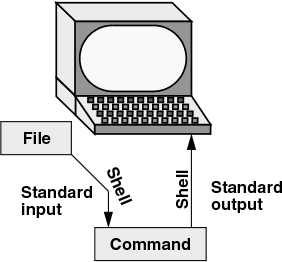
\includegraphics[totalheight=4cm]{/home/anukul/temporary/csc110-project/scrot/fig_stdin}
    \caption{Data flow diagram}
    \label{fig:verticalcell}
\end{figure}

\begin{lstlisting}[language=bash]
$ ./cat File
.....
.....
\end{lstlisting}
The argument File is standard input into the shell to the command and to standard output.\\
Multiple file can be fed into as arguments, files are opened and stdout in order and is outputted together in link of series.

The file hello.txt contains some text. use cat on hello.txt multiple times.
\begin{lstlisting}[language=bash]
$ ./cat hello.txt hello.txt
Hi my name is Anukul.
Hi my name is Anukul.
\end{lstlisting}
\addcontentsline{toc}{section}{Data Flow}
\newpage


\chapter*{Implementation}
\section*{Header Files}
\begin{description}
  \item[$\bullet$ stdlib.h] is for general purpose standard library, which declares a variety of utility functions for type conversions, memory allocation, process control and other similar tasks.
  \item[$\bullet$ stdio.h] defines several macros and declares three types and many functions for performing input and output.
  \item[$\bullet$ string.h] defines macros, constants and declarations of functions and typrs used not only for string handeling but also various memory handling functions.
  \item[$\bullet$ fcntl.h] is the C POSIX library for c programming language that contains constructs that refer to file control.
  \item[$\bullet$ sys/stat.h] is the C POSIX library for c programming language that contains constructs that facilitate getting information about files attributes.
  \item[$\bullet$ unistd.h] defines miscellaneous symbolic constants and types, and declares miscellaneous functions.
  \item[$\bullet$ err.h] defines the integer variable errno, which is set by system call and some library functions of errors to indicate what error is occurring.
\end{description}
\addcontentsline{toc}{chapter}{Implementation}
\addcontentsline{toc}{section}{Header Files}

\newpage
\section*{Functions Used}
\begin{description}
    \item[$\bullet$ int main(int argc, char *argv[]])]
command line arguments is passed, from main function before running program
first argument is the executable file itself and the second one is the argument form user\\
ie. argv[0] holds executable name, argv[1] holds first argument name arguments must be passed with space in between

\item[$\bullet$ fileno()]
the function examines the argument and returns the integer file descriptor.\\
ie. fileno(stdin) returns 0 later useful in program

\item[$\bullet$ strcmp()]
the function compares two strings if: both string are equal it returns 0, negative if first string is les than second string\\
ie. strcmp("hello", "hello") returns 0.

\item[$\bullet$ open()]
the function opens file by specified pathname if not it may create the file in that path
it returns file descriptor greater that 2 because they are 0,1,2 are used by stdin,stdout,stderr
open commonly used flags are O\_RDONLY (read-only), O\_WRONGLY (write-only), O\_RDWR (read/write) these are commonly used file permissions\\
ie. open(*argv, O\_RDONLY) opening pathname given by *argv in readonly mode.

\item[$\bullet$ fstat()]
the function obtains information about file associated with file descriptor and write it to area pointed by buffer.\\
ie. fstat(wfd, \&sbuf) is used to access information from stat structure on wfd.

\item[$\bullet$ malloc()]
the function allocates size bytes and returns a pointer to the allocated memory\\
ie. malloc(bsize) returns pointer to appropriate allocated blocksize

\item[$\bullet$ read()]
the function reads upto bsize bytes from file descriptor to the buffer\\
ie. read(rfd, buf, bsize) the file indicated by rfd is input to memory area indicated by buffer with calculated blocksize

\item[$\bullet$ write()]
the function writes  upto bsize bytes from buffer to file referred by file descriptor.\\
ie. write(wfd, buf, bsize) the file indicated by the wfd is output to the memory area indicated by the buffer with calculated blocksize

\item[$\bullet$ free()]
the function releases allocated memory\\
ie. free(buf) freeing used buffer memory

\item[$\bullet$ close()]
the function closes file descriptor so it no longer refers to any file.\\
ie. close(fd) closing opened file descriptor.


\end{description}
\addcontentsline{toc}{section}{Functions Used}

\section*{Memory Leak \& Performance}
Memory Leak is when memory is allocated and not freed after use, or when the pointer to a memory allocation is deleted, rendering the memory no longer usable. Memory leak degrade performance due to increased paging, and overtime causes a program to crash. When program runs out of memory it may cause Linux kernel to crash.

Compiler doesn't show memory leak so one must use other tools to detect memory leak.
The straightforward way is to use gnu debugger with valgrind both are debugging tool native to linux system.
Detailed memory leak check required some additional compiler arguments.

\begin{lstlisting}[language=bash]
$ gcc -Wall -ggdb3 -o cat cat.c 

\end{lstlisting}
\begin{description}

\item[$\bullet$ ggdb3] produces extra debugging information including macro definitions and line number same as syntax error shows line number in compiler.\\
\end{description}
Debugging took most time and all the issues arised was due to non freed allocated memory. This caused system to crash due to low system memory and larger file size.
Later found out it was due to memory not freed before exiting the program.


\begin{figure}
\centering
        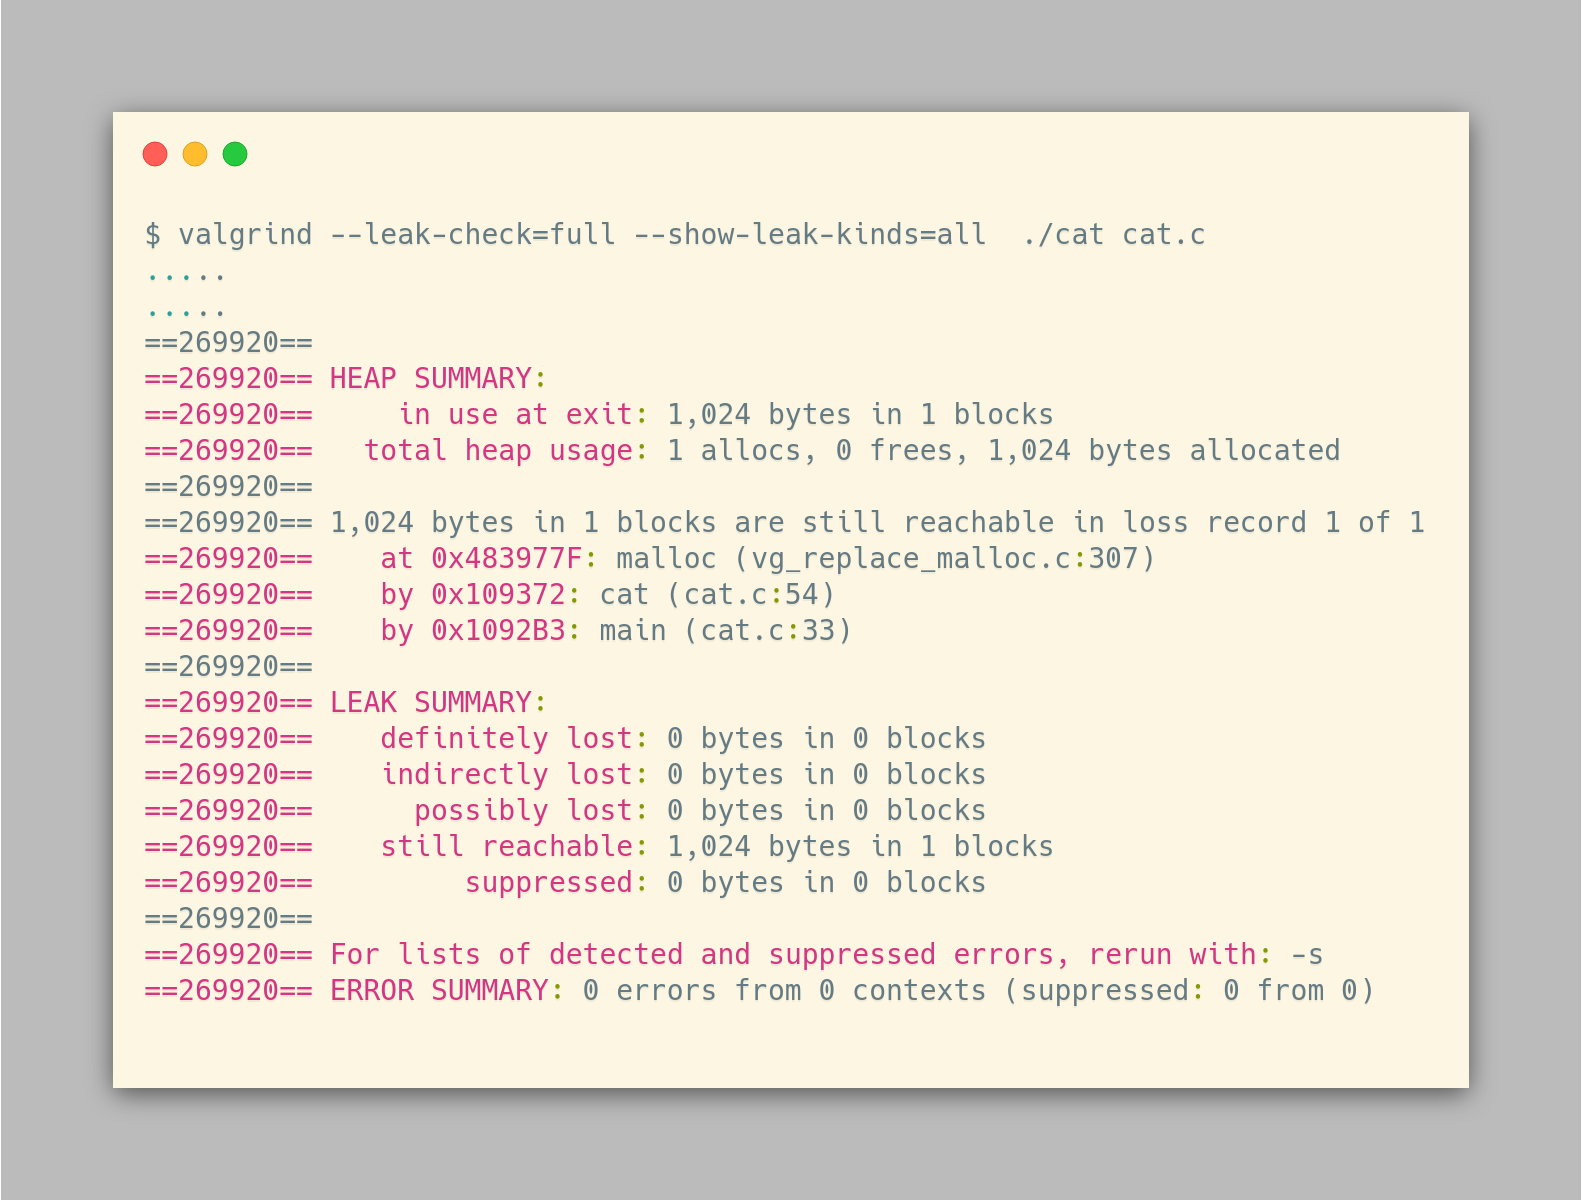
\includegraphics[totalheight=8cm]{/home/anukul/temporary/csc110-project/scrot/mem_leak}
    \caption{Memory Leak caused by not freeing malloc block}
    \label{fig:verticalcell}
\end{figure}

\begin{figure}
\centering
        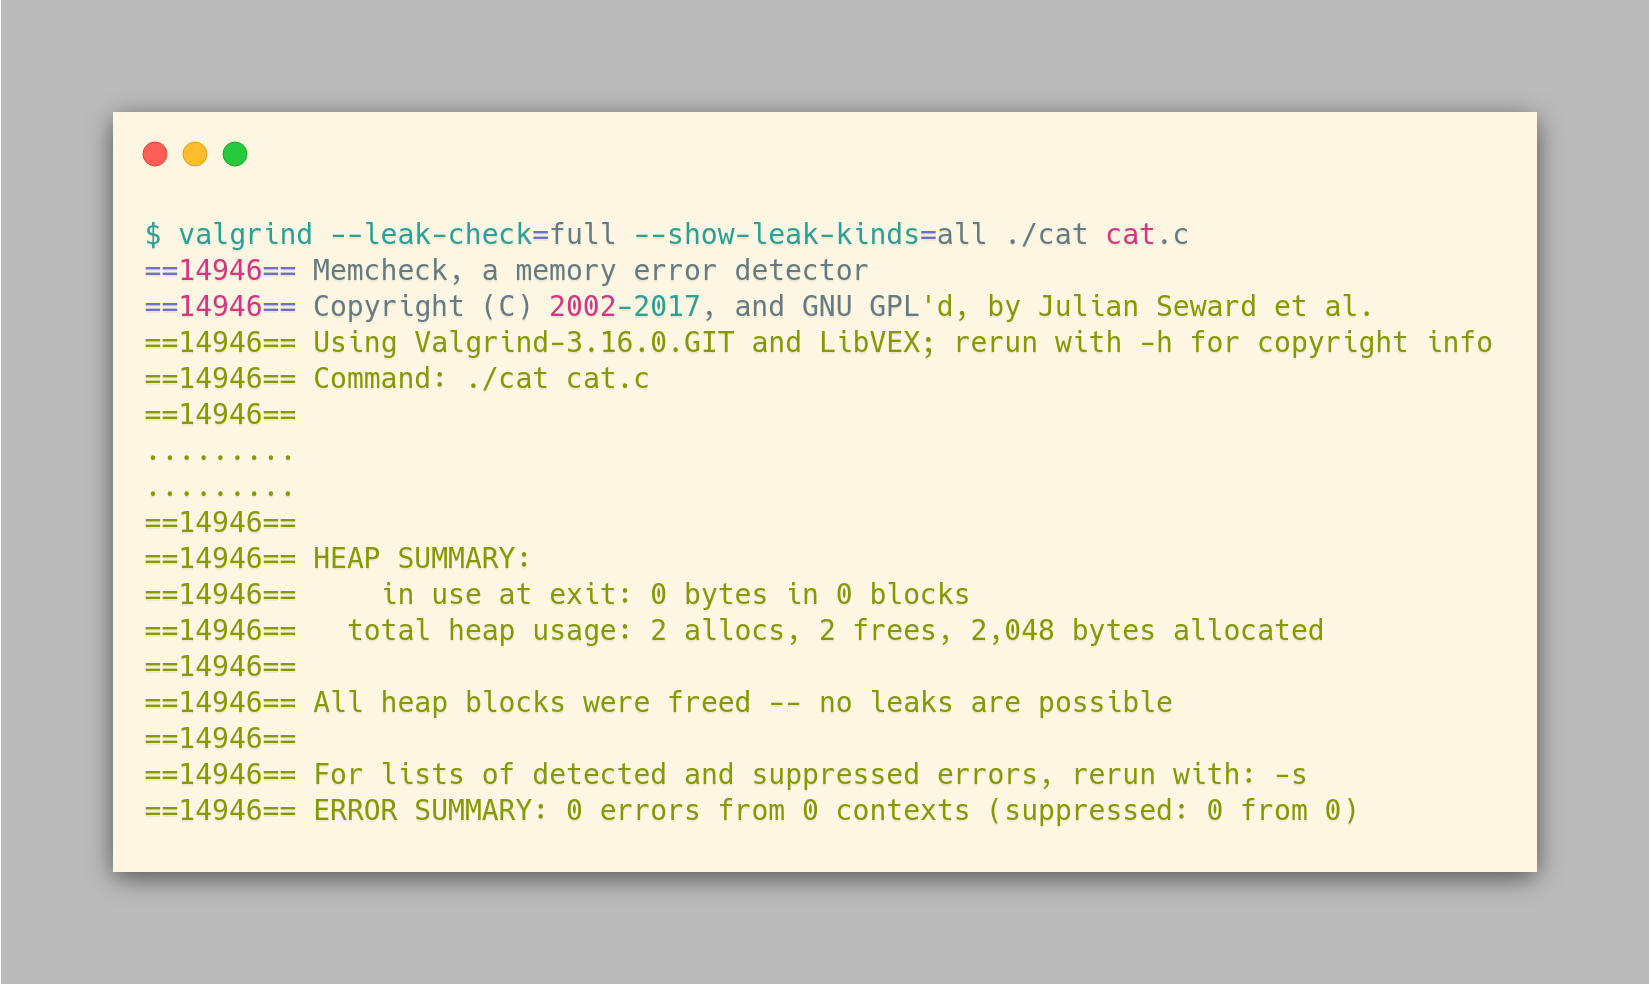
\includegraphics[totalheight=8cm]{/home/anukul/temporary/csc110-project/scrot/fixed_mem_leak}
    \caption{No Memory Leak after freeing malloc block}
    \label{fig:verticalcell}
\end{figure}

        


\addcontentsline{toc}{section}{Memory Leak \& Performance}
\newpage
Lets compare the re-implemented cat and original gnu coreutil cat.\\
\begin{lstlisting}[language=bash]
$ time ./cat cat.c
.................................
.................................

        }
        nr = read(rfd, buf, bsize);
    }
    free(buf);
}

real	0m0.003s
user	0m0.000s
sys	0m0.003s

\end{lstlisting}
\begin{lstlisting}[language=bash]
$ time cat cat.c
.................................
.................................

        nr = read(rfd, buf, bsize);
    }
    free(buf);
}

real	0m0.003s
user	0m0.003s
sys	0m0.000s

\end{lstlisting}

It is \textbf{identical}.

\chapter*{Source Code}
\inputminted{c}{/home/anukul/temporary/csc110-project/src/cat.c}
\addcontentsline{toc}{chapter}{Source Code}
\newpage
\addcontentsline{toc}{chapter}{Bibliography}
\bibliography{references}{}
\bibliographystyle{ieeetr}


\end{document}
